\subsection*{1. Barrier and Queue Tutorial.}
\addcontentsline{toc}{section}{1. Barrier and Queue Tutorial}

\subsubsection{1.1 - Modificar a variável ZK de acordo com a instalação do Zookeeper em run barrier.sh.}
\addcontentsline{toc}{subsection}{1.1 Modificar a variável ZK de acordo com a instalação do Zookeeper em run barrier.sh.}

\vspace{-0.5em}
\begin{minipage}{\textwidth}
  \hspace{-1em}
  \centering
  \lstinputlisting[language=sh]{pratica4/codigos/run_barrier.sh}
  \label{prog1}
  \hspace{1em}
\end{minipage}
\vspace{0.5em}

\subsubsection{1.2 - O que significa a variável SIZE em run barrier.sh?}
\addcontentsline{toc}{subsection}{1.2 O que significa a variável?}
A variável SIZE é o número mínimo de processos filhos para que o nó pai libere a computação de seu processo.

\subsubsection{1.3 - Executar run barrier.sh. O que aconteceu?}
\addcontentsline{toc}{subsection}{1.3 Executar run barrier.sh.}
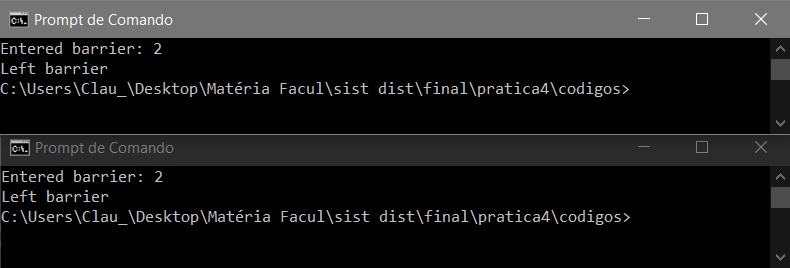
\includegraphics{pratica4/prints/roteiro 1.3.PNG}

\subsubsection{1.4 - Modificar a variável ZK de acordo com a instalação do Zookeeper em
run queue producer.sh.}
\addcontentsline{toc}{subsection}{1.4 Modificar a variável ZK de acordo com a instalação do Zookeeper em
run queue producer.sh.}

\vspace{-0.5em}
\begin{minipage}{\textwidth}
  \hspace{-1em}
  \centering
  \lstinputlisting[language=sh]{pratica4/codigos/run_queue_producer.sh}
  \label{prog1}
  \hspace{1em}
\end{minipage}
\vspace{0.5em}

\subsubsection{1.5 - Modificar a variável ZK de acordo com a instalação do Zookeeper em run queue consumer.sh.}
\addcontentsline{toc}{subsection}{1.5 Modificar a variável ZK de acordo com a instalação do Zookeeper em run queue consumer.sh.}

\vspace{-0.5em}
\begin{minipage}{\textwidth}
  \hspace{-1em}
  \centering
  \lstinputlisting[language=sh]{pratica4/codigos/run_queue_consumer.sh}
  \label{prog1}
  \hspace{1em}
\end{minipage}
\vspace{0.5em}

\subsubsection{1.6 - O que significa a variável SIZE em run queue producer.sh? E em
run queue consumer.sh?}
\addcontentsline{toc}{subsection}{1.6 O que significa a variável SIZE em run queue producer.sh? E em run queue consumer.sh?}
No run queue producer.sh, a variável SIZE corresponde ao número de elementos que serão colocados por ele na fila, enquanto que em run queue consumer, a variável SIZE corresponde ao número de elementos que serão consumidos da fila por ele.


\subsubsection{1.7 - Executar run queue consumer.sh e depois run queue producer.sh.
O que aconteceu? Alterne a execução dos scripts}
\addcontentsline{toc}{subsection}{1.7 Executar run queue consumer.sh e depois run queue producer.sh.}

O processo consumidor fica bloqueado se não houverem elementos para serem consumidos na fila (fica aguardando o produtor inserir esses elementos). Quando os elementos são adicionados ou já existem elementos na fila, o consumidor roda normalmente.\newline


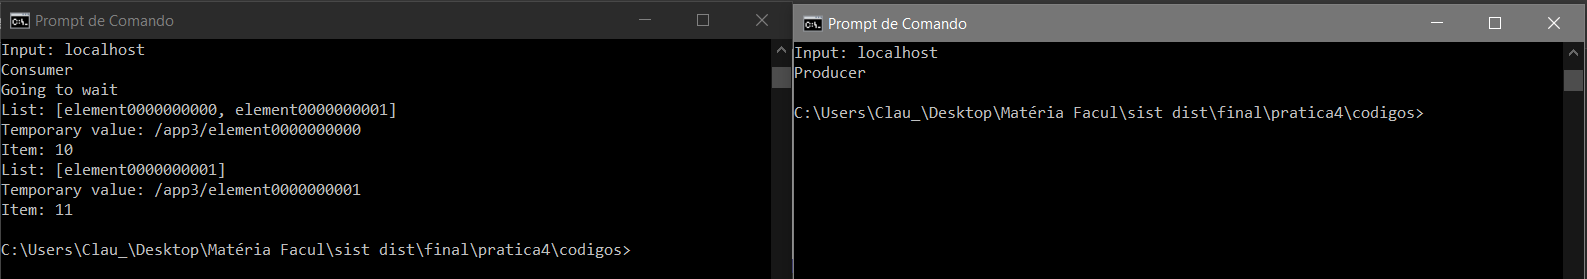
\includegraphics[width=20cm]{pratica4/prints/roteiro 1.7 c-p.PNG}
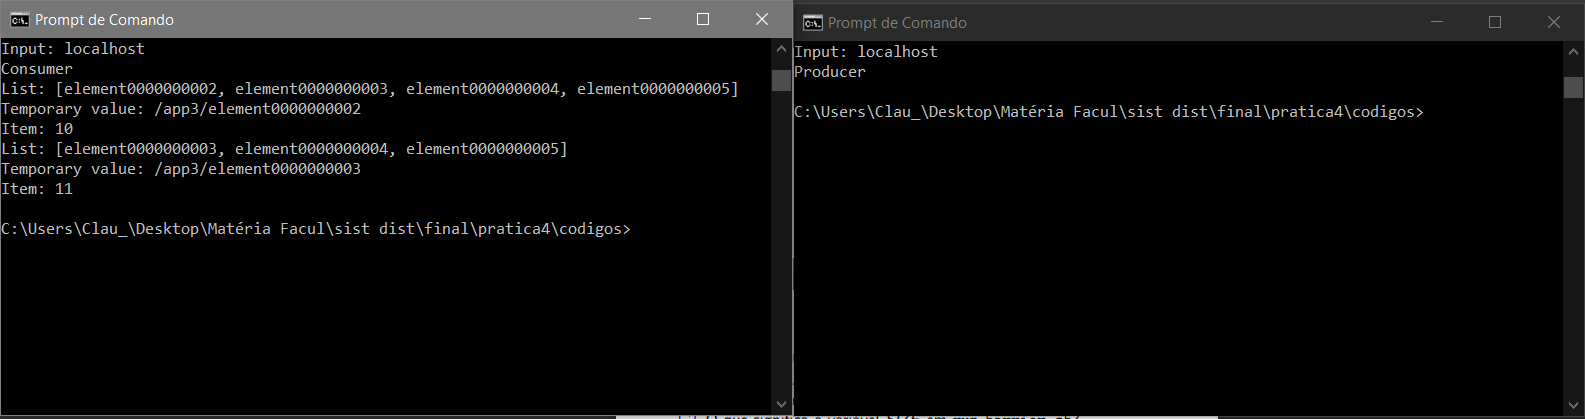
\includegraphics[width=20cm]{pratica4/prints/roteiro 1.7 p-p-c.PNG}

\subsection*{2. Tutorial de lock baseado no Barrier and Queue Tutorial}
\addcontentsline{toc}{section}{2. ?}

\subsubsection{2.1 - Modificar a variável ZK de acordo com a instalação do Zookeeper em run lock.sh.}
\addcontentsline{toc}{subsection}{2.1 Modificar a variável ZK de acordo com a instalação do Zookeeper em run lock.sh.}

\vspace{-0.5em}
\begin{minipage}{\textwidth}
  \hspace{-1em}
  \centering
  \lstinputlisting[language=sh]{pratica4/codigos/run_lock.sh}
  \label{prog1}
  \hspace{1em}
\end{minipage}
\vspace{0.5em}

\subsubsection{2.2 - O que significa a variável WAIT em run lock.sh?}
\addcontentsline{toc}{subsection}{2.2 O que significa a variável WAIT em run lock.sh?}

A variável WAIT corresponde ao tempo de espera para destravar o processo criado com o runlock.sh

\subsubsection{2.3 - Executar várias instâncias de run lock.sh. O que aconteceu?}
\addcontentsline{toc}{subsection}{2.3 Executar várias instâncias de run lock.sh}

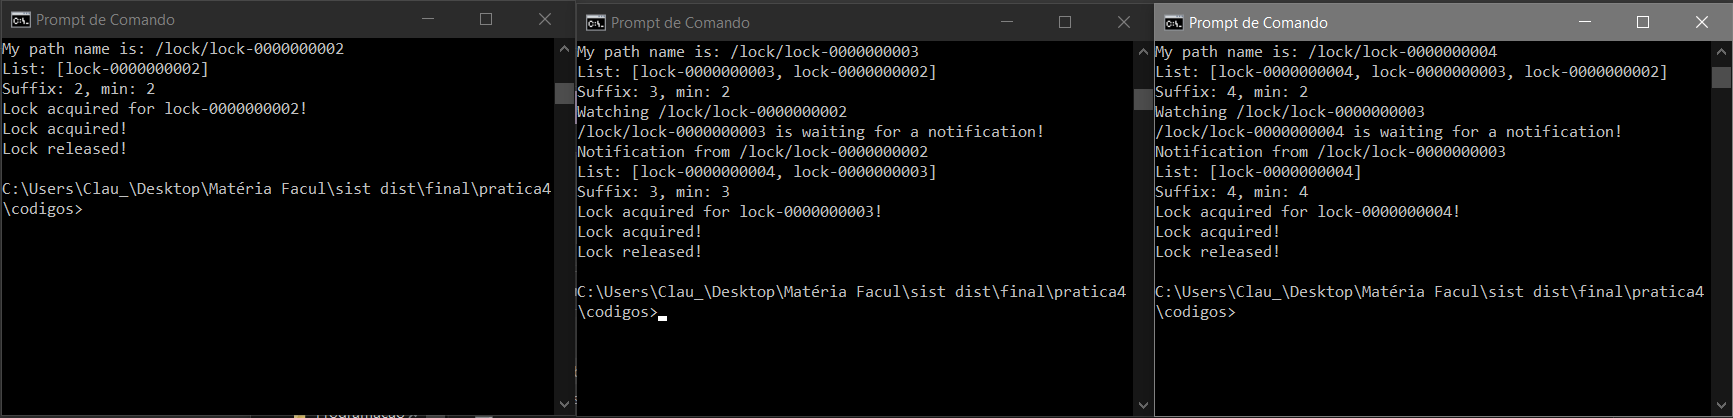
\includegraphics[width=20cm]{pratica4/prints/roteiro 2.3.PNG}

\subsubsection{2.4 - Executar várias instâncias de run lock.sh e, em seguida, matar
alguma instância intermediária. O que aconteceu?}
\addcontentsline{toc}{subsection}{2.4 Executar várias instâncias de run lock.sh e, em seguida, matar alguma instância intermediária}
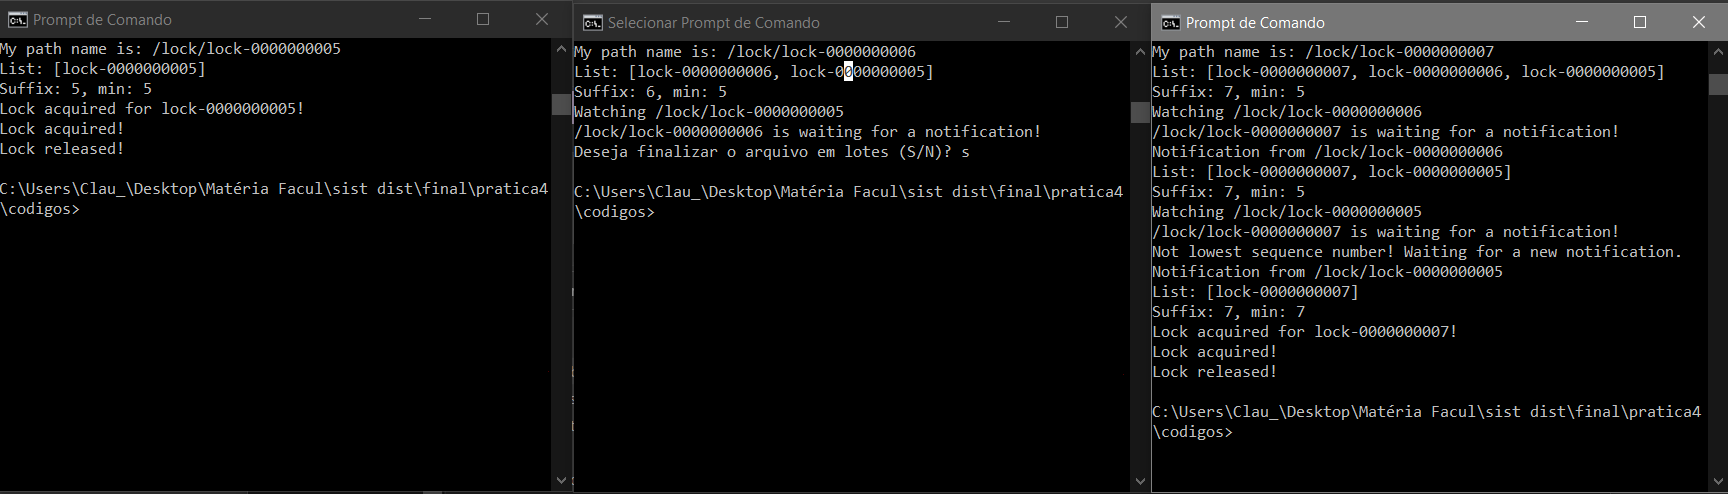
\includegraphics[width=20cm]{pratica4/prints/roteiro 2.4.PNG}